\documentclass[11pt]{article}

\usepackage{amssymb,amsmath,amsthm}
\usepackage{verbatim}
\usepackage{fullpage}
\usepackage{gencor}
\usepackage{mathrsfs}
\numberwithin{equation}{section}
\numberwithin{definition}{section}
\numberwithin{thm}{section}
\numberwithin{lemma}{section}
\numberwithin{prop}{section}
\numberwithin{cor}{section}
\numberwithin{hyp}{section}
\usepackage{graphicx}


\frenchspacing

%\setlength\parindent{0pt}`

\title{Supplementary Note to Estimating Genetic Correlation from GWAS Summary Statistics}
\author{Brendan Bulik-Sullivan}

\begin{document}
\maketitle
\tableofcontents
\newpage

%%%%%%%%%%%%%%%%%%%%%%%%%%%%%%%%%%%%%%%%%%%%%%%%%%%%%%%%%%%%%%%
\section{Definitions}\label{Definitions}
%%%%%%%%%%%%%%%%%%%%%%%%%%%%%%%%%%%%%%%%%%%%%%%%%%%%%%%%%%%%%%%

Let $y_1$ and $y_2$ denote phenotypes defined for individuals in a hypothetical population of infinite size 
(or more precisely, for individuals drawn from a distribution). 
Let $g$ denote a set of additively-coded SNPs, 
and let $g_1$ and $g_2$ denote the best linear predictors of $y_1$ and $y_2$ that can be constructed (at infinite sample size) from the SNPs in $S$\footnote
{Formally, the $g_i$ are constructed by projecting the phenotypes onto the vector space of functions $\{0,1,2\}^M\to\R$, where $M:=|g|.$
As a result $g_i$ may account for a large proportion of the variance in phenotype, 
even if in truth the way in which the phenotype is determined from genotype and environmental factors is completely non-additive.}.
Then we can write
\begin{align*}
	y_1 &= g_1 + \epsilon_1;\\
	y_2 &= g_2 + \epsilon_2,
\end{align*}
where $\epsilon_i$ denotes the residual, which is uncorrelated (in the population) with $g_i$ by the definition of a projection.
Note that so far this construction is applicable to arbitrary phenotypes\footnote{
Well, measurable finite-variance phenotypes. 
But this is no restriction at all on the genetic component, and hardly any restriction at all on the environmental component.}.

\begin{definition}\label{h2}
The narrow-sense (or additive) \textbf{heritability} of phenotype $y_i$ explained by the SNPs in $g$, 
denoted $h^2_g(y_i)$ is defined
\begin{equation}
h^2_g(y_i) := \corr[g_i,y_i]^2,
\end{equation}
\noindent
where $\corr$ denotes the correlation between random variables,
(alternatively, the correlation in a hypothetical population of infinite size),
not the empirical correlation in some finite sample.
\end{definition}

\begin{definition}  
The [additive] \textbf{genetic covariance} between $y_1$ and $y_2$ among SNP set $g$, 
denoted $\rho_g(y_1, y_2)$ is defined
\begin{equation}
\rho_g(y_1, y_2) := \frac{\cov[g_1,g_2]}{\sqrt{\var[y_1]\var[y_2]}}.
\end{equation}
\end{definition}

\begin{definition}  
The [additive] \textbf{genetic correlation} between $y_1$ and $y_2$ among SNP set $g$, 
denoted $r_g(y_1, y_2)$ is defined
\begin{equation}
r_g(y_1, y_2) := \dfrac{\gencov}{\sqrt{h^2_g(y_1)h^2_g(y_2)}}.
\end{equation}
\end{definition}

Note that these definitions make sense even when either or both phenotypes are binary,
and we refer to the specialization of definition \ref{h2} to a binary phenotype as 
the \textbf{\emph{heritability of the observed phenotype}}.

There are two challenges when dealing with binary phenotypes. 
The first is inferential:
often studies of binary phenotypes will over-sample cases in order to increase power.
Some work is required in order to obtain valid estimates of the parameters of a population with, say, 1\% cases 
from an ascertained sample with 50\% cases.
Ascertainment is addressed in section \ref{Conditional Expectation, Case/Control Traits}.
The second challenge is definitional: the heritability of the observed phenotype depends strongly on the prevalence of the
phenotype. 
For example, consider two liability threshold phenotypes $y_1$ and $y_2$, 
determined by the same underlying liability $\psi$, but with different thresholds. 
That is, $y_i := \mathbf{1}[\psi > \tau_i]$ for $i=1,2$.
Suppose $h^2_g(\psi)=1$, $\tau_1 = 0$ and $\tau_2 = 1.96$ 
(meaning the population prevalence of $y_1$ is 50\% and the population prevalence of $y_2$ is 5\%),
then the heritability of the observed phenotype $y_1$ is $0.64$,
and the heritability of the observed phenotype $y_2$ is $0.23$.

Sometimes it is desirable to compare the heritabilities or genetic covariances of phenotypes with different prevalences on an even footing,
and this is the primary application of liability-scale heritability and liability scale genetic covariance.
We note that one need not take the liability threshold model literally\footnote{We also note that the liability threshold model is (trivially) completely general. Let $y$ denote an arbitrary binary phenotype with prevalence $K$, and set $\tau := \Phi^-{1}(1-K)$, where $\Phi$ is the cdf of the standard normal distribution. We can construct a liability for $y$ as follows: if individual $i$ is a case, draw a liability $\psi_i$ from a truncated standard normal with left truncation point $\tau$. If individual $i$ is a control, draw a liability $\psi_i$ from a truncated standard normal with right truncation point $\tau$. Then $y=\mathbf{1}[\psi > \tau]$.}
in order for the conversion to the liability scale to be a useful procedure.
One can view this conversion simply as a tool for comparing phenotypes with different prevalences that is inspired by --
but not dependent on -- the liability threshold model.
An interpretation of LD Score regression under the liability threshold model is provided in section \ref{}.

There is no need to specify a scale when discussing genetic correlation. 
Genetic correlation on the observed scale is the same as genetic correlation on the liability scale is the same as genetic correlation in an ascertained sample.
	
%%%%%%%%%%%%%%%%%%%%%%%%%%%%%%%%%%%%%%%%%%%%%%%%%%%%%%%%%%%%%%%
\section{Models}
\subsection{Quantitative Traits}\label{ctsmodel}
%%%%%%%%%%%%%%%%%%%%%%%%%%%%%%%%%%%%%%%%%%%%%%%%%%%%%%%%%%%%%%%

Suppose we sample two cohorts for two phenotypes,
$y_1$ and $y_2$,
with sample sizes $N_1$ and $N_2$,
such that $N_s$ individuals are shared between cohorts and phenotyped for both traits.
We model phenotypes as generated by the equations
\begin{align*}
	y_1 &= Y\beta + \delta;\\
	y_2 &= Z\gamma + \epsilon,
\end{align*}
where $Y$ and $Z$ are matrices of genotypes normalized to mean zero and variance one\footnote{
We ignore the distinction between normalizing and centering in the population and in the sample, 
since this introduces only $\mathscr{O}(1/N)$ error.},
with dimensions $N_1\times M$ and $N_2\times M$, respectively; 
$\beta$ and $\gamma$ are $M\times 1$ vectors of per-normalized genotype effect sizes,
and $\delta$ and $\epsilon$ are vectors of environmental or non-additive genetic effects,
with dimensions $N_1\times 1$ and $N_2\times 1$, respectively.
In this model, $Y$ and $Z$ are unobserved matrices of \emph{all} SNPs,
unlike Yang, \emph{et al} \cite{yang2010}, 
we model the effects of SNPs that are not genotyped as well as those that are.

Now we introduce randomness:
we model all of $Y, Z, \beta, \gamma, \delta $ and $\epsilon$ as random variables.
Suppose that the $2M\times1$ vector $(\beta, \gamma)$ follows a distribution with mean zero and variance-covariance matrix\
\begin{equation*} 
	\var[(\beta, \gamma)] = \frac{1}{M}
		\left( \begin{array}{cc}
		\hsqo I & \gencov I\\
		\gencov I& \hsqt  I
	\end{array} \right),
\end{equation*}
and the $2N\times1$ vector $(\delta, \epsilon)$ follows a distribution with mean zero and variance-covariance matrix
\begin{equation*}
	\var[(\delta, \epsilon)] = 
		\left( \begin{array}{cc}
		(1-\hsqo) I & \envcov I\\
		\envcov I& (1-\hsqt) I
	\end{array} \right).
\end{equation*}
Finally suppose that each row (individual) of $Y$ and $Z$ 
represents an \emph{i.i.d.} draw from a distribution with covariance matrix (LD matrix) $R$
(except of course the $N_s$ rows that are duplicated in $Y$ and $Z$).
We will write $\E[Y_{ij}Y_{ik}] = R_jk =: r_jk$. 
Note that since we assume normalized genotypes,
$R$ is both the covariance matrix and correlation matrix. 
Additionally, note that under this model, $\var[y_1] = \var[y_2] = 1$. 
Let $\rho := \gencov + \envcov$ denote the covariance between $y_1$ and $y_2$,
which is also the correlation between $y_1$ and $y_2$, since both have variance one.

The assumption that all $\beta$ is drawn with equal variance for all SNPs is, of course, not reasonable.
We only make this assumption here for notational simplicity. 
In this paper, we use MAF- and LD-partitioned LD Score regression for estimation, as described in references \cite{finucane2014partitioning,buliksullivan2014kernel}.
This technique minimizes confounding under models where $\var[\beta]$ is correlated with MAF or LD Score.


\begin{prop} Under this model, the expected genetic covariance between phenotypes is $\gencov$, justifying our use of the notation $\gencov$.
\end{prop}
\begin{proof} Let $X$ denote an $1\times M$ vector of normalized, centered genotypes for an arbitrary individual. 
Under the model, the additive genetic component of $y_1$ for this individual is $\sum_j X_j\beta_j$,
and the additive genetic component of $y_2$ for this individual is $\sum_j X_j\gamma_j$.
Thus, the genetic covariance between $y_1$ and $y_2$ is 
$$\cov\left[\sum_{j=1}^M X_j\beta_j,\sum_{j=1}^M X_j\gamma_j\right],$$ 
\noindent
We can simplify this covariance with some algebra:
\begin{align*}
	\cov\left[\sum_{j=1}^M X_j\beta_j,\sum_{j=1}^M X_j\gamma_j\right] &= 
		\E\left[\left(\sum_{j=1}^M X_j\beta_j\right)\left(\sum_{j=1}^M X_j\gamma_j\right)\right]\\
		&= \E\left[ \sum_{j=1}^M \sum_{k=1}^M X_jX_j\beta_j\gamma_k\right]\\
		&= \E\left[ \sum_{j=1}^M X_j^2\beta_j\gamma_j \right]\\
		&= \sum_{j=1}^M \E[X_j^2]\E[\beta_j\gamma_j]\\
		&= \rho_g.
\end{align*}
\end{proof}

%%%%%%%%%%%%%%%%%%%%%%%%%%%%%%%%%%%%%%%%%%%%%%%%%%%%%%%%%%%%%%%
\subsection{Liability Threshold Model}
%%%%%%%%%%%%%%%%%%%%%%%%%%%%%%%%%%%%%%%%%%%%%%%%%%%%%%%%%%%%%%%

Suppose unobserved liability is generated following the usual model for quantitative traits:
\begin{equation*}
	\psi_i = \sum_{j=1}^M X_{ij}\beta_j + \epsilon_i.
\end{equation*}
The observed binary phenotype has population prevalence $K$, 
and is generated from the unobserved liability via the liability threshold model:
\[
	y_i := \ind[\psi_i > \tau],
\]
where $\tau:=\Phi^{-1}(1-K)$ is the liability threshold, and
$\Phi$ denotes the cdf of the standard normal distribution.

%%%%%%%%%%%%%%%%%%%%%%%%%%%%%%%%%%%%%%%%%%%%%%%%%%%%%%%%%%%%%%%
\section{Derivations}
%%%%%%%%%%%%%%%%%%%%%%%%%%%%%%%%%%%%%%%%%%%%%%%%%%%%%%%%%%%%%%%

\subsection{Non-Ascertained Samples}
\subsubsection{Genetic Covariance}
\label{supp_condexp_qt}
Suppose we directly genotype SNP $j$. 
We estimate effect sizes using least-squares: 
\begin{align*}
	\bhat_j &:= \frac{1}{N_1}\T{Y}_jy_1;\\
	\chat_j &:= \frac{1}{N_2}\T{Z}_jy_2,
\end{align*}
where $Y_j$ and $Z_j$ denote the genotypes of all individuals at SNP $j$ 
and have dimensions $N_1\times 1$ and $N_2\times 1$, respectively.

\begin{prop} 
Under the model described in \ref{ctsmodel}, 
\begin{equation}
	\E[\bhat_j\chat_j] = \frac{\gencov}{M}\ell_j  + \frac{N_s\rho}{N_1N_2}.
\end{equation}
\end{prop}

\begin{proof} By the law of total expectation, 
$$\E[\bhat_j\chat_j] = \E[ \E[\bhat_j\chat_j \,|\, Y, Z ] ]$$
\noindent
First,
\begin{align*}
	\E[\bhat_j\chat_j\,|\,Y,Z] &= \frac{1}{N_1N_2}\E[\T{Y}_jy_1\T{y_2}Z_j]   \\
       		&= \frac{1}{N_1N_2}\T{Y}_j\E[{(Y\beta+\delta)}(Z\gamma+\epsilon)]Z_j\\
        		&= \frac{1}{N_1N_2}\T{Y}_j\left(Y\E[\beta\T{\gamma}]Z + \E[\T{\delta}\epsilon]\right)Z_j\\
        		&= \frac{1}{N_1N_2}\left( \frac{\gencov}{M} \T{Y}_jY\T{Z}_jZ  + \envcov\T{Y}_jZ_j  \right).
\end{align*}
\noindent
To remove the conditioning on $Y$ and $Z$, we need only compute 
$$\frac{1}{N_1N_2}\E[\T{Y}_jZ_j ] = \frac{N_s}{N_1N_2},$$ 
and 
$$\frac{1}{N_1N_2}\E[\T{Y}_jY\T{Z}_jZ] = \ell_j + \frac{MN_s}{N_1N_2}.$$
Thus, 
\begin{align*}
    \E[\bhat_j\chat_j] &= \frac{\gencov}{M}\ell_j  + \frac{N_s\rho}{N_1N_2}.
\end{align*}
Note that this expression does not contain any terms in which both the quantities $N_s$ and $\ell_j$ appear. 
In the special case where there are no overlapping samples shared between the two cohorts, this expression simplifies to 
\begin{equation*}
	\E[\bhat\chat] = \frac{\gencov}{M}\ell_j.
\end{equation*}
\end{proof}

%%%%%%%%%%%%%%%%%%%%%%%%%%%%%%%%%%%%%%%%%%%%%%%%%%%%%%%%%%%%%%%
\subsubsection{Regression Weights}
%%%%%%%%%%%%%%%%%%%%%%%%%%%%%%%%%%%%%%%%%%%%%%%%%%%%%%%%%%%%%%%

We can improve the efficiency of the LD Score regression by computing the conditional variance 
$\var[\bhat\chat \,|\,\ell_j]$
and weighting the regression by the reciprocal of this variance. 
In order to compute this conditional variance, 
we need further assumptions: in addition to the assumptions from \ref{ctsmodel}, 
assume that the phenotypes follow a multivariate normal distribution\footnote{
For instance, it is sufficient but not necessary to assume that $\beta$, $\gamma$, $\delta$ and $\epsilon$ are multivariate normal, 
and that $N_1$ and $N_2$ are sufficiently large that we can invoke the central limit theorem. 
More generally, the phenotypes will be approximately normal if $\delta$ and $\epsilon$ are normal 
and if $\beta$ and $\gamma$ are reasonably polygenic.
If there are few casual SNPs, then the conditional variance may be larger.}.

If phenotypes are normally distributed, then by the central limit theorem,
$\bhat$ and $\chat$ are jointly normally distributed with expectation zero. 
Thus,
\begin{align}
    \var[\bhat_j\chat_j\,|\,Y,Z] 
&= 
	\E[\bhat^2\chat^2]\nonumber\\
&=  
	\var[\bhat]\var[\chat]
	+
	2\E[\bhat\chat]^2\nonumber\\
&= 
	\left( 
		\frac{\hsqo\ell_j}{M} 
		+ 
		\frac{1}{N_1} 
	\right) \left(  
		\frac{\hsqt\ell_j}{M} 
		+ 
		\frac{1}{N_2}
	\right) 
	+ 					
	2\left( 
		\frac{\gencov\ell_j}{M} 
		+ 
		\frac{\rho N_s}{N_1N_2} 
	\right)^2.
\end{align}

Note that we only assume normality in order to compute regression weights.
If (quantitative) phenotypes are not normally distributed,
this will not affect the expectation of the LD Score regression estimates
(see \ref{supp_condexp_qt}, which makes no distributional assumptions about $\beta$ and $\gamma$ beyond first and second moments),
but will increase the standard error,
because in this case the regression weights will not be optimal for correcting for heteroskedasticity.
We never assume homoskedasticity when computing standard errors or $p$-values 
(we use a block jackknife, which is robust to heteroskedasticity), 
so non-normality of the phenotypes also does not bias our inference.
We derive regression weights for ascertained studies of binary phenotypes in section \ref{supp_condvar_cca}.
Note that if the phenotypes are normally distributed, then $\bhat_j\chat_j$
follows a product-normal distribution, which is not in the exponential family, so this is not a GLM.

%%%%%%%%%%%%%%%%%%%%%%%%%%%%%%%%%%%%%%%%%%%%%%%%%%%%%%%%%%%%%%%
\subsection{Ascertainment}
%%%%%%%%%%%%%%%%%%%%%%%%%%%%%%%%%%%%%%%%%%%%%%%%%%%%%%%%%%%%%%%

In this section, we derive the LD Score regression estimators of heritability and genetic covariance for ascertained case/control
samples (which was addressed only via simulation in \cite{buliksullivan2014}).
The fact that this estimator works is \emph{not} a consequence of the equivalence between LD Score regression and HE 
regression (see section \ref{LD Score Regression is Haseman-Elston Regression}),
and the fact that HE regression works in ascertained case/control samples \cite{golan2013narrowing},
because case/control ascertainment induces LD between causal SNPs in the ascertained samples. 
HE regression accounts for this LD by using a GRM computed from sample genotypes. 
It is not clear \emph{a priori} that the LD Score regression approach of using population LD as an estimate of sample LD
is valid when the sample is ascertained.
However, this turns out to be fine,
though we do not address this issue directly.
Our proof strategy is first to note that GWAS summary statistics can be written in terms of the sample allele frequencies in cases and the sample allele frequencies
in controls. 
Since the sample allele frequency in cases is a consistent estimator of the population allele frequency in cases, and likewise for the sample allele frequency in controls, 
we can write the large-$N$ limit of our GWAS summary statistics in terms of the population allele frequencies (see section \ref{CCA:Case/Control Test Statistics}).
Since the population allele frequencies depend on population LD rather than ascertained sample LD, LD Score regression with population LD yields a consistent
estimators of heritability and genetic covariance.

This section is structured as follows: 
in \ref{CCA:Heritability} and \ref{CCA:Genetic Covariance}, 
we show that using estimates of population LD is a valid, even with ascertained samples,
and we derive the usual factors for converting heritabilities and genetic covariances from ascertained samples into
estimates of the population heritabilities and genetic covariances.

In \ref{CCA:Liability Threshold Model}, we deal with the special case of the liability threshold model, and derive LD Score 
regression estimators of the heritability of liability, and genetic covariance between liability and other phenotypes.


%%%%%%%%%%%%%%%%%%%%%%%%%%%%%%%%%%%%%%%%%%%%%%%%%%%%%%%%%%%%%%%
\subsubsection{Case/Control Test Statistics}\label{CCA:Case/Control Test Statistics}
%%%%%%%%%%%%%%%%%%%%%%%%%%%%%%%%%%%%%%%%%%%%%%%%%%%%%%%%%%%%%%%


Consider a study of size $N$ where the sample prevalence of phenotype $y$ is $P$. 
Let $N_{eff} := NP(1-P) = N_0N_1/N $ denote the effective sample size.
We compute $Z$-statistics
\begin{equation}
\label{z}
Z_j := 
\frac
	{\sqrt{N_{eff}}(\hat{p}_1 - \hat{p}_0)} 
	{\sqrt{\hat{p}_j(1-\hat{p}_j)}},
\end{equation}
and
$\chi^2$-statistics\footnote{
This is the equal to $N$ times the squared correlation between phenotype and genotype,
\emph{i.e.,} the Armitage Trend Test (ATT).}
\begin{equation}
\label{chisq}
	\chi^2_j := Z_j^2,
\end{equation}
where $\hat{p}_j$ denotes allele frequency in the entire sample\footnote{
Note that if $j$ has nonzero effect size, the expected value of $\hat{p}_j$ is not equal to $p_j$ 
unless $P=K$.},
$\hat{p}_1$ denotes allele frequency among cases in the sample
and $\hat{p}_0$ denotes allele frequency among controls in the sample.
We aim to derive an estimator of heritability from $\E[\chi^2_j\cond\ell_j]$ and an estimator of genetic covariance from $\E[Z_j\cond\ell_j]$ 
in samples where $P\neq K$ under various models of genetic architecture.
First, we need a lemma, which allows us to write our $\chi^2$-statistics in terms of population allele frequencies in the large-$N$ limit.

\begin{lemma}
In an ascertained study with sample size $N$, sample prevalence $P$ and population prevalence $K$, the expected $Z$-statistic of a SNP $j$
conditional on its population allele frequencies in cases and controls is
\begin{equation}
	\E[Z_j\cond p_0,p_1] =
\end{equation}
and the expected $\chi^2$ statistic is
\begin{equation}
	\E[\chi^2_j\cond p_0,p_1] = +1.
\end{equation}
\end{lemma}
\begin{proof}

Note that the case where we condition on $p_0$ and $p_1$ 
(\emph{i.e.,} when the only randomness is from sampling and genetic architecture is nonrandom),
is the usual case considered in power analyses for GWAS, so we can even obtain the asymptotic distributions of
the $Z$ and $\chi^2$ statistics from standard results on Wald statistics.
First,
\begin{equation*}
	Z_j\cond p_0, p_1 \sim N()
\end{equation*}
so
\begin{equation*}
	\E[Z_j\cond p_0,p_1] =
\end{equation*}
and $\chi^2_j$ follows a noncentral $\chi^2$ distribution with one degree of freedom and non-centrality parameter
\begin{equation*}
	\mathrm{NCP} =
\end{equation*}
Since the expected value of a noncentral $\chi^2$ distribution with $k$ degrees of freedom and noncentrality parameter $\lambda$ is 
$k+\lambda$,
\begin{equation*}
	\E[\chi^2_j\cond p_0, p_1] = +1
\end{equation*}
\end{proof}

%%%%%%%%%%%%%%%%%%%%%%%%%%%%%%%%%%%%%%%%%%%%%%%%%%%%%%%%%%%%%%%
\subsubsection{Heritability of the Observed Phenotype}\label{CCA:Heritability}
%%%%%%%%%%%%%%%%%%%%%%%%%%%%%%%%%%%%%%%%%%%%%%%%%%%%%%%%%%%%%%%




Next, we remove the conditioning on $p_0$ and $p_1$ by noting that 
$p_0$ and $p_1$ are fixed conditional on $\beta_{loc}$,
and can be approximated using \ref{taylor1} and \ref{taylor2}.
Thus, the inner term of the numerator from \ref{totalexp} is
\begin{align}
\label{numerator2}
\notag
	\E[(\hat{p}_1 -\hat{p}_0)^2\cond\beta_{loc}]
\approx
	\dfrac{p_j^2\phi(\tau)^2\alpha_j^2}{K^2(1-K)^2}
&+
	\dfrac{p_j(1-p_j)
	+
	\dfrac{p_j\phi(\tau)\alpha_j}{K}\left(
	1 - 2p_j - \dfrac{p_j\phi(\tau)\alpha_j}{K}	
	\right)}{N_1}\\
&+	
	\dfrac{p_j(1-p_j)
	+
	\dfrac{p_j\phi(\tau)\alpha_j}{K}\left(
	2p_j -1 - \dfrac{p_j\phi(\tau)\alpha_j}{K}	
	\right)}{N_0}.\nonumber\\
&\approx
	 \dfrac{p_j^2\phi(\tau)^2\alpha_j^2}{K^2(1-K)^2} + \mathscr{O}(1/N).
\end{align}




Next, we remove the conditioning on $p_0$ and $p_1$. 
Let $C:=\phi(\tau)P(1-K) + K(1-P))/(K(1-K))$. 
Using the approximations from \ref{taylor1} and \ref{taylor2},
\begin{align*}
	\tilde{p}_j\cond\beta_{loc}
&\approx
	p_j\left(
		1 + C\alpha_j
	\right),
\end{align*}
and
\begin{align*}
	\E[\tilde{p}_j(1-\tilde{p}_j)\cond\beta_{loc}]
&=
	p_j(1 + C\alpha_j)(1-p_j-p_jC\alpha_j)\\
&=
	p_j\left(
		1-p_j+C\alpha_j(1-2p_j-p_jC\alpha_j).
	\right).
\end{align*}
Note that we have already computed $p_0(1-p_0)\cond\beta_{loc}$
and $p_1(1-p_1)\cond\beta_{loc}$ in \ref{numerator2}.
Thus, the inner term of the denominator of \ref{totalexp} is
\begin{align}
\label{denom}
\notag
	\E[\hat{p}_j(1-\hat{p}_j)\cond\beta_{loc}]
&= 
	p_j\left(
		1-p_j+C\alpha_j(1-2p_j-p_jC\alpha_j)
	\right)\\\notag
&-
	\dfrac{(1-P)^2p_j(1-p_j)
	+
	\dfrac{p_j\phi(\tau)\alpha_j}{K}\left(
	2p_j -1 - \dfrac{p_j\phi(\tau)\alpha_j}{K}	
	\right)}{N_0}\\
&-
	\dfrac{P^2p_j(1-p_j)
	+
	\dfrac{p_j\phi(\tau)\alpha_j}{K}\left(
	1 - 2p_j - \dfrac{p_j\phi(\tau)\alpha_j}{K}	
	\right)}{N_1}\nonumber\\
&\approx
	p_j\left(
		1-p_j+C\alpha_j(1-2p_j-p_jC\alpha_j)
	\right) + \mathscr{O}(1/N).
\end{align}

We now introduce randomness into $\beta$. 
For this section, model the entries of $\beta$ as \emph{i.i.d.} draws 
from a distribution with expectation zero and variance $h^2/M$.
The heritability of liability (in the population) under this model is $h^2$; 
$\E[\alpha_j]=0$;
$\E[Z_j]=0$, and 
\[
	\E[\alpha_j^2] = \frac{(1-p_j)h^2}{p_jM}\ell_j.
\]
The expected numerator of the $\chi^2$-statistic is therefore
\begin{align*}
	N_{eff}\E[(\hat{p}_1 - \hat{p}_0)^2]
&=
	p_j(1-p_j)\left(\dfrac{N_{eff}\phi(\tau)^2h^2\ell_j}{K^2(1-K)^2M}
	\left(
		1
		+
		\dfrac{N(1-K)^2}{N_0N_1K^2}
	\right)
	+
	\dfrac{NN_{eff}}{N_0N_1}
	\right)\\
&\approx
	p_j(1-p_j)\left(\dfrac{N_{eff}\phi(\tau)^2h^2\ell_j}{MK^2(1-K)^2}
	+
	1\right),
\end{align*}
where the approximation is justified by the fact that $N/N_0N_1 \ll1$,
which is a reasonable approximation when $P$ is not so far from $1/2$ (a balanced study).
For brevity, let $c$ denote
\[
	c := \dfrac{P(1-P)\phi(\tau)^2}{K^2(1-K)^2},
\]
which is the factor used to convert between liability scale heritability, $h^2$ and observed scale heritability, $h^2_{obs} := ch^2$.

The expected denominator of the $\chi^2$-statistic is 
\begin{align*}
	\E[\hat{p}_j(1-\hat{p}_j)]
&=
	p_j(1-p_j) -\mathscr{O}(\ell_j/M)+\mathscr{O}(1/N)\\
&\approx
	p_j(1-p_j).
\end{align*}
Thus,
\begin{align}
	\E[\chi^2_j]
&\approx
	c\dfrac{Nh^2}{M}\ell_j+1\nonumber\\
&=
	\dfrac{Nh^2_{obs}}{M}\ell_j+1.
\end{align}


%%%%%%%%%%%%%%%%%%%%%%%%%%%%%%%%%%%%%%%%%%%%%%%%%%%%%%%%%%%%%%%
\subsubsection{Genetic Covariance with the Observed Phenotype}\label{CCA:Genetic Covariance}
%%%%%%%%%%%%%%%%%%%%%%%%%%%%%%%%%%%%%%%%%%%%%%%%%%%%%%%%%%%%%%%

In this section, we derive a genetic covariance estimator that works when both studies are ascertained to oversample cases and may include overlapping samples.
This derivation does not cover more complicated ascertainment schemes 
(\emph{e.g.,} attempting to estimate genetic covariance between T2D and BMI from a T2D GWAS consisting of low-BMI cases 
and high-BMI controls).


%%%%%%%%%%%%%%%%%%%%%%%%%%%%%%%%%%%%%%%%%%%%%%%%%%%%%%%%%%%%%%%
\subsubsection{Heritability and Genetic Covariance of Liability}\label{CCA:Liability Threshold Model}
%%%%%%%%%%%%%%%%%%%%%%%%%%%%%%%%%%%%%%%%%%%%%%%%%%%%%%%%%%%%%%%

For phenotypes generated according to the liability threshold model, we can estimate not only the heritability of the observed
phenotype (genetic covariance between the observed phenotype and other phenotypes), but also the heritability of the 
unobserved liability (genetic covariance between unobserved liability and other phenotypes).

The derivation is the same as in \ref{CCA:Heritability} and \ref{CCA:Genetic Covariance}, except with one extra step: 
we need to write $\prob[y_i=1\cond G_{ij}=1]$ in terms of the heritability of liability.

Let $\alpha_j:=\E[\psi\cond G_{ij}=1] = p_j^{-\frac{1}{2}}(1-p_j)^{\frac{1}{2}}\sum_{\{k\cond r_{jk} \neq 0\}} r_{jk}\beta_k$ 
denote the marginal per-normalized genotype effect size of SNP $j$ on liability.
This is the per-normalized-genotype effect size that one would obtain from regressing liability against the genotype at SNP $j$
at infinite sample size.

Then if $\phi(x,\mu,\sigma^2)$ denotes the density of a normal distribution
with expectation $\mu$ and variance $\sigma^2$ evaluated at $x$,
\begin{align*}
	\prob[y_i=1\cond G_{ij}=1] 
&= 
	\int_{\tau}^\infty \phi(x,\alpha_j,1-\alpha_j^2)dx\\
&=
	\int_{\tau-\alpha_j}^\infty \phi(x(1-\alpha_j^2)^{\frac{1}{2}};0,1)dx\\
&= % u = x\sqrt{1-\alpha_j^2}
	(1-\alpha_j^2)^{-\frac{1}{2}}\int_{(\tau-\alpha_j)(1-\alpha_j^2)^{\frac{1}{2}}}^\infty \phi(u;0,1)du\\
&= 
	(1-\alpha_j^2)^{-\frac{1}{2}}(1 - \Phi(\tau')),
\end{align*}
where $\tau' := (\tau-\alpha_j)(1-\alpha_j^2)^{\frac{1}{2}}$. 
Similarly,
\begin{align*}
	\prob[y_i=0\cond G_{ij}=1] 
&= 
	1-\prob[y_i=1\cond G_{ij}=1] \\
&=	
	1 - (1-\alpha_j^2)^{-\frac{1}{2}}(1 - \Phi(\tau')).
\end{align*}

We approximate $\Phi(\tau')$ with a first-order Taylor expansion\footnote{
This is a reasonable approximation for small $\alpha_j$, \emph{e.g.,} for polygenic traits
and away from loci with huge effects.}
around $\tau$:
\begin{align*}
	\Phi(\tau') 
&\approx 
	\Phi(\tau) + \phi(\tau)(\tau'-\tau)\\
&=
	1-K + \phi(\tau)(\tau'-\tau).
\end{align*}
We also make the approximation that
$$(1-\alpha_j^2)^{\frac{1}{2}}\approx 1.$$
Thus we have
\begin{align}
\label{taylor1}
\notag
	p_1\cond\beta_{loc} 
&= 
	\dfrac{p_j}{K}(1-\alpha_j^2)^{-\frac{1}{2}}(1 - \Phi(\tau'))\\
&\approx
	p_j\left(1+\frac{\phi(\tau)\alpha_j}{K}\right),
\end{align}
and
\begin{align}
\label{taylor2}
\notag
	p_0\cond\beta_{loc} 
&=  
	\frac{p_j}{1-K}\left(
		1 - (1-\alpha_j^2)^{-\frac{1}{2}}(1 - \Phi(\tau'))
	\right)\\
&\approx
	p_j\left(1 - \frac{\phi(\tau)\alpha_j}{1-K}\right).
\end{align}

We can plug these results into the expressions from \ref{CCA:Heritability} in order to obtain an estimator of the heritability
of liability:
 
 WRITE MEEEE

%%%%%%%%%%%%%%%%%%%%%%%%%%%%%%%%%%%%%%%%%%%%%%%%%%%%%%%%%%%%%%%
\subsubsection{Regression Weights}\label{CCA:Regression Weights}
%%%%%%%%%%%%%%%%%%%%%%%%%%%%%%%%%%%%%%%%%%%%%%%%%%%%%%%%%%%%%%%

Lorem Ipsum Dolor Sic Amet

%%%%%%%%%%%%%%%%%%%%%%%%%%%%%%%%%%%%%%%%%%%%%%%%%%%%%%%%%%%%%%%
\section{LD Score Regression is Haseman-Elston Regression}\label{LD Score Regression is Haseman-Elston Regression}
%%%%%%%%%%%%%%%%%%%%%%%%%%%%%%%%%%%%%%%%%%%%%%%%%%%%%%%%%%%%%%%

In this section we re-interpret LD Score regression as an approximation to Haseman-Elston (HE) regression \cite{haseman1972}
that is valid for samples of unrelated individuals. 
In section \ref{HE:Heritability}, we prove equivalence between a modified LD Score estimator of heritability and HE regression,
and and in section \ref{HE:Genetic Covariance} we prove equivalence between and modified LD Score estimator of 
genetic covariance and HE regression.
In section \ref{The Local LD Approximation}, we describe the interpretation of standard LD Score regression as an approximation
to HE regression, and some of the advantages of this approximation, in particular, the ability to model all SNPs, not just 
genotyped SNPs, and robustness to population stratification.


%%%%%%%%%%%%%%%%%%%%%%%%%%%%%%%%%%%%%%%%%%%%%%%%%%%%%%%%%%%%%%%
\subsection{Heritability}\label{HE:Heritability}
%%%%%%%%%%%%%%%%%%%%%%%%%%%%%%%%%%%%%%%%%%%%%%%%%%%%%%%%%%%%%%%

Suppose we condition on the matrix of sample genotypes $X$
(which is a matrix encoding normalized and centered genotypes at \emph{all} SNPs),
but otherwise follow the univariate version of the model in \ref{ctsmodel} (\emph{i.e.,} the model in \cite{buliksullivan2014}).
Then the variance-covariance matrix of the $N\times 1$ vector $y$ of phenotypes is
\begin{equation*}
	\var[y]  =  h^2_gA + (1-h^2_g)I,
\end{equation*}
where $A := \T{X}X/M$ is the sample GRM. 
This means that $\E[y_hy_i] = h^2_g A_{hi}/M$,
so we can estimate genetic covariance by regressing $y_hy_i$ against $A_{hi}$
and multiplying by the slope by $M$.
Precisely,
\begin{equation}
	\hat{h}^2_{g,HE} :=  \frac{M\covhat[A_{hi}, y_hy_i]}{\varhat[A_{hi}]},
\end{equation}
where $\varhat$ and $\covhat$ denote sample variance and sample covariance, respectively.
This estimator is called Haseman-Elston (HE) regression \cite{haseman1972}.

There is another LD Score-based estimator of heritability, 
the aggregate estimator:	
\begin{align}
	\hat{h}^2_{g, agg} 
&:= 
	\frac{1}{\lbar}_{sample}\sum_{j=1}^M \chi^2_j\\
&\approx
	\frac{1}{\lbar}\sum_{j=1}^M (\chi^2_j-1)
\end{align}
where $\lbar := \mean_j(\ell_j)$. We should call attention to a notational choice: we can choose to deal with the $\mathscr{O}(1/N)$
upward bias in sample $r^2$ by subtracting one from $\chi^2$ and using $\lbar$, the mean population LD Score,
or by not subtracting one from $\chi^2$ and using $\lbar_{sample}$, the mean LD Score in our (finite) sample.
Recall from the supplementary note of \cite{buliksullivan2014} that we have the relationship
\begin{equation}
	\lbar_{sample} \approx \lbar + \dfrac{M}{N}
\end{equation}
in an unstructured sample.
Since for this section we are assuming that we have access to raw genotypes, we deal with $\lbar_{sample}$.
We discuss the implications of approximating sample LD Score with an estimate of population LD Score from a sequenced reference panel 
in \ref{The Local LD Approximation}.

\begin{prop}\label{agg}

The aggregate estimator is an unbiased estimate of heritability, and is
equivalent to the LD Score regression estimator with the intercept constrained to zero\footnote{
Note that a consequence of constraining the intercept is that the aggregate estimator, 
unlike the LD Score regression estimator, is not immune to population stratification or cryptic relatedness.} (if using sample LD Score)
or constrained to one (if using population LD Score).

\end{prop}
\begin{proof}
This follows immediately from the supplementary note of \cite{buliksullivan2014}.
\end{proof}
Note that computing these estimators requires raw genotypes at all SNPs, 
which is generally only possible with sequence data.
Often geneticists substitute a GRM computed using only genotyped SNPs. 
The distinction is unimportant for this derivation; for now, fix a set of observed SNPs $j=1,\ldots,M_g$. 
We discuss the distinction between using all SNPs and only genotyped SNPs in section \ref{The Local LD Approximation}.

\begin{prop}\label{he_vs_agg}
Let $\rhat_{jk}$ denote the sample correlation between SNPs $j$ and $k$ in matrix $X$
Let 
$$\lhat_j := \sum_{j=1}^{M_g} \rhat_{jk}^2$$
denote sample LD Score in $YX$
with the sum taken only over the $M_g$ observed SNPs.
Let $\lbar_{X}$ denote the mean value of $\lhat_{j}$ among genotyped SNPs $j=1,\ldots,M_g$.
If we use this version of $\lbar$ for the denominator of the aggregate estimator, 
then the aggregate estimator is equal to the HE estimator. 
\end{prop}

\begin{proof} The numerator of the HE estimator is 
\begin{align*}
	M\covhat[A_{hi}, y_hy_i] 
&= 
	\frac{M}{N^2}
		\sum_{h=1}^{N} 
			\sum_{i=1}^{N} 
				A_{hi}y_hy_i	\\
&= 
	\frac{1}{N^2} 
		\sum_{h = 1}^{N} 
			\sum_{i = 1}^{N} 
				\sum_{j = 1}^M 
					X_{hi}X_{ij}y_hy_i	 \\
&= 
	\frac{1}{N^2}\sum_{j = 1}^M \left( 
		\sum_{h = 1}^{N} 
			\sum_{i = 1}^{N} X_{hj}
				y_1 X_{ij}y_2 
	\right) \\
&= 
	\sum_{j = 1}^M \chi^2_j.
\end{align*}	
The denominator of the HE estimator is 
\begin{align*}
	\varhat[A_{hi}]
&= 
	\frac{1}{N^2} 
		\sum_{h = 1}^{N}
			\sum_{i = 1}^{N} 
				A_{hi}^2\\
&= 
	\frac{1}{MN^2} 
		\sum_{h = 1}^{N} 
			\sum_{i = 1}^{N} \left( 
				\sum_{j = 1}^M 
					X_{hj}X_{ij} 
			\right)^2\\
&= 
	\frac{1}{MN^2} 
		\sum_{h = 1}^{N}	
			\sum_{i = 1}^{N}
				\sum_{j = 1}^M 
					\sum_{k=1}^M 
						X_{hj}X_{hk}X_{ij}X_{ik} \\	
&= 
	\frac{1}{M} 
		\sum_{j = 1}^M \left( 
			\sum_{k=1}^M \rhat_{jk}^2
		\right),\\
&= 
	\frac{1}{M} 
		\sum_{j=1}^M 
			\lhat_j \\
&= 
	\lbar_{X}.
\end{align*}
Since the numerator of the HE estimator is equal to the numerator of the aggregate estimator 
and the denominator of the HE estimator is equal to the denominator of the aggregate estimator,
the conclusion follows.  \\
\end{proof}

%%%%%%%%%%%%%%%%%%%%%%%%%%%%%%%%%%%%%%%%%%%%%%%%%%%%%%%%%%%%%%%
\subsection{Genetic Covariance}\label{HE:Genetic Covariance}
%%%%%%%%%%%%%%%%%%%%%%%%%%%%%%%%%%%%%%%%%%%%%%%%%%%%%%%%%%%%%%%

The proof of the equivalence between the LD Score aggregate estimator of genetic covariance and the HE regression estimator 
of genetic covariance is a direct bivariate analogue of the proof of the equivalence of the LD Score aggregate heritability 
estimator in the HE regression heritability estimator from \ref{HE:Heritability}; however, we present the proof in full detail for
reference. For notational simplicity, we assume no sample overlap in this section. 

Suppose we condition on $Y$ and $Z$
(which are matrices encoding genotypes at \emph{all} SNPs),
but otherwise follow the model in \ref{ctsmodel}.
Then the variance-covariance matrix of the $(N_1+N_2)\times 1$ vector $(y_1,y_2)$ of phenotypes is
\[
	\var[(y_1,y_2)]  =  \frac{1}{M} \left( \begin{array}{cc}
		\hsqo Y\T{Y}      &  \gencov Y\T{Z} 	\\
		\gencov Z\T{Y}  &  \hsqt Z\T{Z}
	\end{array} \right)
	+
	\left( \begin{array}{cc}
		(1-\hsqo)I & 0 	\\
		0              & (1-\hsqt)I
	\end{array} \right).
\]
Let $A := \T{Y}Z/M$. 
This means that $\E[y_{1h}y_{2i}] = \gencov A_{hi}$,
so we can estimate genetic covariance by regressing $y_{1h}y_{2i}$ against $A_{hi}$ and multiplying the slope by $M$.
This is a bivariate analogue of HE) regression first introduced (to the best of our knowledge) in \cite{price2011}.
The estimator is
\begin{equation}
	\hat{\rho}_{g,HE} :=  \frac{M\covhat[A_{hi}, y_{1h}y_{2i}]}{\varhat[A_{hi}]},
\end{equation}
where $\varhat$ and $\covhat$ denote sample variance and sample covariance, respectively.

There is another LD Score-based estimator of genetic correlation, 
the aggregate estimator:	
\begin{equation}
	\hat{\rho}_{g, agg} := \frac{1}{\lbar}\sum_{j=1}^M \bhat_j\chat_j,
\end{equation}
where $\lbar := \mean_j(\ell_j)$.
\begin{prop}\label{agg}
The aggregate estimator is an unbiased estimate of genetic covariance, and is
equivalent to the LD Score regression estimator with the intercept constrained to zero\footnote{
Note that a consequence of constraining the intercept to zero is that the aggregate estimator, 
unlike the LD Score regression estimator, is not immune to sample overlap.}. 

\end{prop}
\begin{proof}
For unbiasedness,
\begin{align*}
	\E[\hat{\rho}_{g,agg}]
&= 
	\frac{1}{\lbar} \sum_{j=1}^M \E[\bhat_j\chat_j]\\
&=
	\frac{1}{\lbar} \sum_{j=1}^M \frac{\gencov}{M}\ell_j\\
&=
	\gencov.
\end{align*}

If we constrain the LD Score regression intercept to zero,
then the LD Score regression slope is equal to the slope of the line connecting the origin to the point
$(\lbar, \mean_j[\bhat_j,\chat_j])$, which is 
$\mean_j[\bhat_j,\chat_j]) / \lbar$.
The LD Score regression estimate of genetic covariance is $M$ times this slope, 
which is equal to the aggregate estimate.
\end{proof}

Note again that computing these estimators requires raw genotypes at all SNPs, 
which is generally only possible with sequence data.
Often geneticists substitute a GRM computed using only genotyped SNPs. 
The distinction is unimportant for this derivation; for now, fix a set of observed SNPs $j=1,\ldots,M_g$. 
We discuss the distinction between using all SNPs and only genotyped SNPs in section \ref{The Local LD Approximation}.

\begin{prop}\label{he_vs_agg_h2}
Let $\rhat_{Y,jk}$ denote the sample correlation between SNPs $j$ and $k$ in matrix $Y$, and likewise for $\rhat_{Z,jk}$.
Let 
$$\lhat_{YZ,j} := \sum_{j=1}^{M_g} \rhat_{Y,jk}\rhat_{Z,jk} $$ 
denote sample LD Score in $Y$ and $Z$ with $r^2_{jk}$ estimated as $\rhat_{Y,jk}\rhat_{Z,jk}$,
(which is an unbiased estimate in the absence of sample overlap)
and the sum taken only over the $M_g$ genotyped SNPs.
Let $\lbar_{YZ}$ denote the mean value of $\lhat_{YZ,j}$ among genotyped SNPs $j=1,\ldots,M_g$.
If we use this version of $\lbar$ for the denominator of the aggregate estimator, 
then the aggregate estimator is equal to the HE estimator. 
\end{prop}

\begin{proof} The numerator of the HE estimator is 
\begin{align*}
	M\covhat[A_{hi}, y_{ih}y_{2i}] 
&= 
	\frac{M}{N_1N_2}
		\sum_{h=1}^{N_1} 
			\sum_{i=1}^{N_2} 
				A_{hi}y_{1h}y_{2}	\\
&= 
	\frac{1}{N_1N_2} 
		\sum_{h = 1}^{N_1} 
			\sum_{i = 1}^{N_2} 
				\sum_{j = 1}^M 
					Y_{hj}Z_{ij}y_{1h}y_{2i}	 \\
&= 
	\frac{1}{N_1N_2}\sum_{j = 1}^M \left( 
		\sum_{h = 1}^{N_1} 
			\sum_{i = 1}^{N_2} Y_{hj}
				y_{1h} Z_{ij}y_{2i} 
	\right) \\
&= 
	\sum_{j = 1}^M \bhat_j\chat_j.
\end{align*}	
The denominator of the HE estimator is 
\begin{align*}
	\varhat[A_{hi}]
&= 
	\frac{1}{N_1N_2} 
		\sum_{h = 1}^{N_1}
			\sum_{i = 1}^{N_2} 
				A_{hi}^2\\
&= 
	\frac{1}{MN_1N_2} 
		\sum_{h = 1}^{N_1} 
			\sum_{i = 1}^{N_2} \left( 
				\sum_{j = 1}^M 
					Y_{hj}Z_{ij} 
			\right)^2\\
&= 
	\frac{1}{MN_1N_2} 
		\sum_{h = 1}^{N_1}	
			\sum_{i = 1}^{N_2}
				\sum_{j = 1}^M 
					\sum_{k=1}^M 
						Y_{hj}Z_{hk}Y_{ij}Z_{ik} \\	
&= 
	\frac{1}{M} 
		\sum_{j = 1}^M \left( 
			\sum_{k=1}^M \rhat_{Y,jk}\rhat_{Z,jk} 
		\right),\\
&= 
	\frac{1}{M} 
		\sum_{j=1}^M 
			\lhat_{YZ,j} \\
&= 
	\lbar_{YZ}.
\end{align*}
Since the numerator of the HE estimator is equal to the numerator of the aggregate estimator 
and the denominator of the HE estimator is equal to the denominator of the aggregate estimator,
the conclusion follows.  \\
\end{proof}
\begin{cor} The HE regression estimator of genetic correlation is equivalent to the LD Score regression estimate obtained 
from regressing\footnote{
Since this is not the optimal weighting for LD Score regression, 
it follows that the aggregate estimator should be more efficient than HE regression,
so long as the LD Scores are estimated with reasonable accuracy.}
$\bhat_j\chat_j$ against $\lhat_{YZ,j}$ with the intercept constrained to zero.
\end{cor}
\begin{proof}
This follows from propositions \ref{agg} and  \ref{he_vs_agg}.
\end{proof}

%%%%%%%%%%%%%%%%%%%%%%%%%%%%%%%%%%%%%%%%%%%%%%%%%%%%%%%%%%%%%%%
\subsection{Local LD}\label{The Local LD Approximation}
%%%%%%%%%%%%%%%%%%%%%%%%%%%%%%%%%%%%%%%%%%%%%%%%%%%%%%%%%%%%%%%

Finally, we can interpret ordinary LD Score regression with LD Scores estimated from a sequenced reference panel
as a modification of HE regression with a GRM computed from all SNPs. 
We state this interpretation in terms of the heritability estimators; the corresponding statements for the genetic covariance estimators
are directly analogous.
The approximation consists of observing that although the equality $\varhat[A_{hi}]=\lbar_X$ holds exactly only when $\lbar_X$ is computed using a
whole-genome window (\emph{i.e.,} including LD across chromosomes), all real LD is local, and all non-local LD results from
finite sample bias in $\hat{r}^2$ or sample structure, so we can write
\begin{equation}\label{local ld eqn}
	\hat{\ell}_j \approx \ell_j + \dfrac{M}{N} + a,
\end{equation}
where $\hat{\ell}_j$ denotes the sample LD Score for SNP $j$, and $a$ is a term that depends on sample structure \cite{buliksullivan2014}.
This approximation justifies replacing $\hat{\ell}_j$ and $\lbar_X$ with an unbiased estimate of population LD Score 
($\ell_j$) from a sequenced reference panel. This approximation step provides several advantages:
\begin{enumerate}
	\item The computational complexity of LD Score regression is much lower than HE regression. HE regression requires time
	$\mathscr{O}(M_gN^2)$ for computing the GRM and $\mathscr{O}(N^2)$ for the regression. LD Score regression requires
	time $\mathscr{O}(MN_{ref})$ for computing LD Scores (times a constant factor $B\approx 5000$,
	the mean window size measured in number of SNPs), where $N_{ref}$ is the sample size of the sequenced reference panel,
	$\mathscr{O}(MN)$ for computing summary statistics\footnote{It almost doesn't seem fair to count the time it takes to compute summary statistics towards the time complexity of LD Score regression, since computing summary statistics is the first thing that every GWAS consortium does.},
	 and time $O(M_g)$ for the regression. 
	Thus, HE regression is quadratic in $N$, and LD Score regression is linear\footnote{If instead of local LD, we had used 
	genome-wide LD, the complexity of estimating LD Scores would have been $\mathscr{O}(M^2N)$, which is intimidating.}. 
	
	\item Using a sequenced reference panel for estimating LD Scores allows us to model the effects of all SNPs in the reference panel,
	not just those SNPs that are directly genotyped or well-imputed in our GWAS sample.
	
	\item The LD Score regression intercept, which results from the approximation \ref{local ld eqn} is a term that depends on sample structure, 
	confers robustness to population stratification and cryptic relatedness (or sample
	overlap, in the case of the genetic covariance estimator). In contrast, HE regression does not know the difference between ``real" 
	LD and spurious LD induced by sample structure (though of course if one has the genotypes, it is easy to fix this problem by including
	principal components as covariates \cite{price2006principal}).
 	
\end{enumerate}


\newpage
\section{Supplementary Figures}
\subsection{Comparison of Metabolic Genetic Correlations from LDSC to Results from Vattikuti, et al}
\begin{figure}[!ht]

\begin{centering}
%\caption{S}
    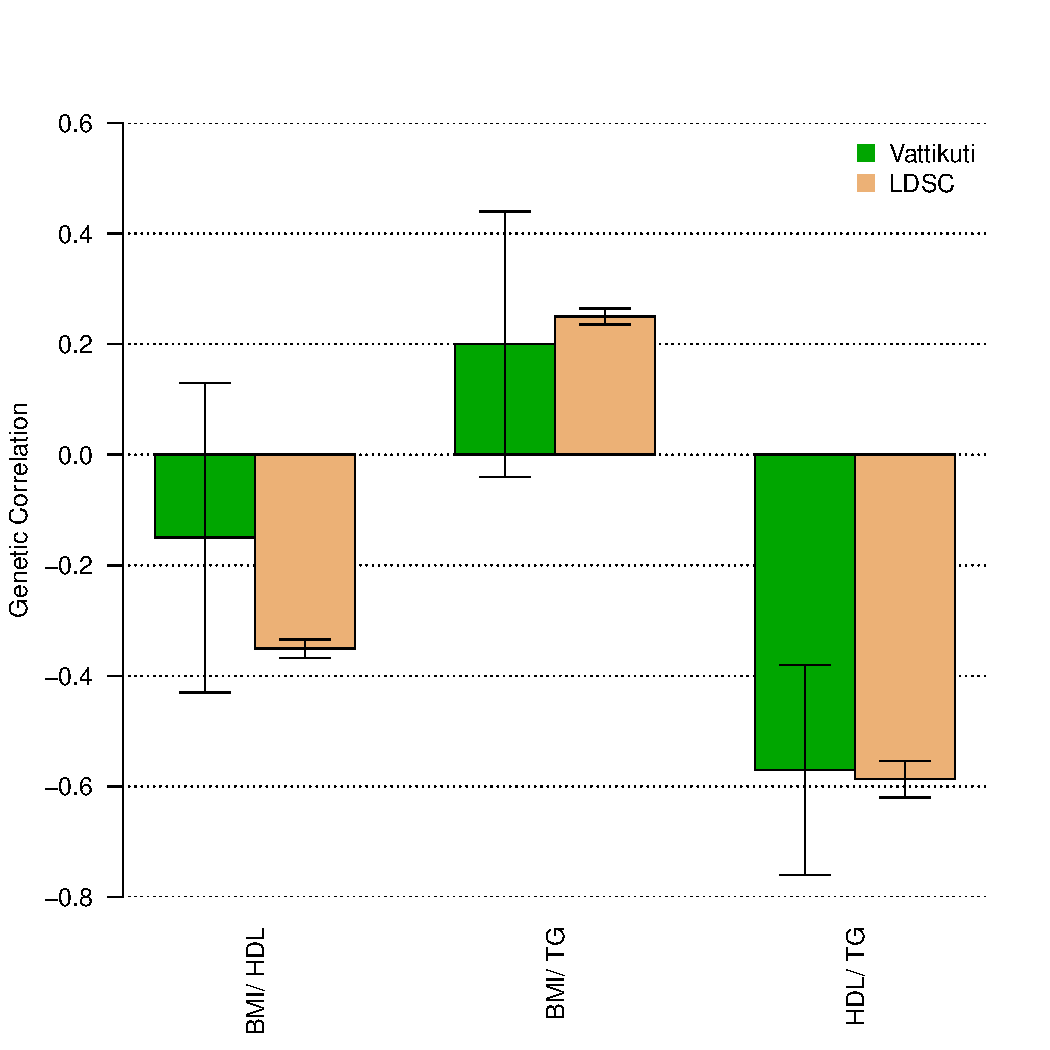
\includegraphics[scale=0.8]{figs/vattikuti.pdf}
         \label{vattikuti}

This figure compares the estimates of genetic correlations between metabolic traits from table 3 of \cite{vattikuti2012heritability}
to the results obtained using roughly 10x larger sample sizes and LD Score regression in this paper.
\end{centering}
\end{figure}

\newpage
\section{Supplementary Tables}

\subsection{Simulations with Parallel LD- and MAF-Dependence}
\label{parallel}
% latex table generated in R 3.1.0 by xtable 1.7-3 package
% Sat Oct 11 21:28:47 2014
\begin{table}[ht]
\centering
\begin{tabular}{llll}
  \hline
LD Score & $h^2(5\myhyphen50\%)$ & $\rho_g(5\myhyphen50\%)$ & $r_g(5\myhyphen50\%)$ \\ 
  \hline
Truth & 0.83 & 0.42 & 0.5 \\ 
  HM3 & 0.53 (0.08) & 0.28 (0.07) & 0.52 (0.1) \\ 
  PNG & 0.36 (0.08) & 0.18 (0.06) & 0.5 (0.13) \\ 
  30 Bins & 0.81 (0.12) & 0.41 (0.08) & 0.51 (0.09) \\ 
  60 Bins & 0.81 (0.12) & 0.41 (0.09) & 0.51 (0.09) \\ 
   \hline
\end{tabular}
\end{table}

This table displays simulations with MAF- and LD-dependent genetic architecture where the MAF- and LD- dependence was the same for both phenotypes and genetic correlation did not vary with MAF or LD. Precisely, effect sizes were drawn from a normal distribution so that the magnitude of per-allele effect sizes were uncorrelated with MAF and variants with LD Score below 100 were $4\times$ enriched for heritability.

In all simulations, the sample size was 2062 individuals with full sample overlap between studies; the causal SNPs were best-guess imputed 1000 Genomes SNPs on chromosome 2, and the SNPs retained for the LD Score regression were HapMap 3 SNPs. 

Estimates are averages across 100 simulations. Standard deviations (in parentheses) are calculated as the empirical standard deviation across 100 simulations.

LD Scores were estimated using in-sample LD and a 1cM window. 
HM3 LD Score is $\sum r^2$ with the sum taken over SNPs in HapMap 3. 
The PNG LD Score is $\sum r^2$ with the sum taken over all SNPs in 1kG as in \cite{buliksullivan2014}. The 30 bins LD Score is a per-allele LD Score binned on a MAF by LD Score grid with MAF breaks at 0.05, 0.1, 0.2, 0.3 and 0.4 and LD Score breaks at 35, 75, 150 and 400. The 60 bins LD Score is a per-allele LD Score binned on a MAF by LD Score grid with MAF breaks at 0.05, 0.1, 0.15, 0.2, 0.25, 0.3, 0.35, 0.4 and 0.45 and LD Score breaks at 30, 60, 120, 200 and 300

These simulations demonstrate that naive LD Score regression can give accurate genetic correlation estimates even in situations where the heritability and genetic covariance estimates are badly biased, so long as genetic correlation does not depend on MAF or LD. In addition, these simulations demonstrate that MAF- and LD-binned LD Score regression can give accurate estimates of heritability and genetic covariance even for genetic architectures with MAF- and LD-dependence.

\newpage
\subsection{Simulations with Antiparallel LD- and MAF-Dependence}
\label{antiparallel}
% latex table generated in R 3.1.0 by xtable 1.7-3 package
% Fri Aug 22 16:49:51 2014
\begin{table}[ht]
\centering
\begin{tabular}{lllll}
  \hline
LD Score & $h^2_1(5\myhyphen50\%)$ & $h^2_2(5\myhyphen50\%)$ & $\rho_g(5\myhyphen50\%)$ & $r_g(5\myhyphen50\%)$ \\ 
  \hline
Truth & 0.83 & 0.89 & 0.33 & 0.38 \\ 
  Naive & 0.36 (0.08) & 1.13 (0.08) & 0.32 (0.07) & 0.5 (0.09) \\ 
  30 Bins & 0.8 (0.14) & 0.93 (0.12) & 0.34 (0.11) & 0.39 (0.1) \\ 
  60 Bins & 0.79 (0.14) & 0.93 (0.12) & 0.33 (0.11) & 0.39 (0.1) \\ 
   \hline
\end{tabular}
\end{table}

This table displays simulations with MAF- and LD-dependent genetic architecture where the MAF- and LD- dependence was in opposite directions for each phenotype, and genetic correlation did not vary with MAF or LD. Precisely, per-allele effect sizes for the first phenotype were drawn from a normal distribution so that the variance of per-allele effect sizes were uncorrelated with MAF, and variants with LD Score below 100 were $4\times$ enriched for heritability. Per-allele effect sizes for the second phenotype were drawn from a normal distribution so that the variance of per-allele effect size followed $\sqrt{p(1-p)}$, where $p$ is MAF, and variants with LD Score above 100 were $4\times$ enriched for heritability. Otherwise, the parameters of these simulations were the same as in \ref{parallel}
These simulations demonstrate that naive LD Score regression can give approximately accurate genetic correlation estimates even in situations where the heritability and genetic covariance estimates are badly biased, so long as genetic correlation does not depend on MAF or LD. In addition, these simulations demonstrate that MAF- and LD-binned LD Score regression can give accurate estimates of heritability and genetic covariance even for genetic architectures with MAF- and LD-dependence.
\newpage
\subsection{Simulations with LD- and MAF-Dependent Genetic Correlation}
\label{depcor}
% latex table generated in R 3.1.0 by xtable 1.7-3 package
% Fri Aug 22 16:49:51 2014
\begin{table}[ht]
\centering
\begin{tabular}{lllll}
  \hline
LD Score & $h^2_1(5\myhyphen50\%)$ & $h^2_2(5\myhyphen50\%)$ & $\rho_g(5\myhyphen50\%)$ & $r_g(5\myhyphen50\%)$ \\ 
  \hline
Truth & 0.83 & 0.89 & 0.41 & 0.48 \\ 
  Naive & 0.38 (0.07) & 1.15 (0.08) & 0.5 (0.06) & 0.75 (0.06) \\ 
  30 Bins & 0.81 (0.1) & 0.94 (0.13) & 0.42 (0.1) & 0.48 (0.09) \\ 
  60 Bins & 0.81 (0.12) & 0.94 (0.13) & 0.42 (0.1) & 0.48 (0.09) \\ 
   \hline
\end{tabular}
\end{table}


In these simulations, effect sizes for the first phenotype were drawn from a normal distribution with mean zero and variance
$(pq)^{0.6}(1+\mathrm{log}(\ell_j)/50)^2$, 
effect sizes for the second phenotype were drawn form a normal distribution with mean zero and variance
$(pq)^{0.3}(1-\mathrm{log}(\ell_j)/50)^2$,
then noise following a normal distribution with mean zero and variance 
$ 1+(7-1)\ell_j/700$,
was added to the effect sizes for the second phenotype, so that genetic correlation was roughly 0.35 for low LD SNPs and 
0.65 for high LD SNPs.   

%This table displays simulations with MAF- and LD-dependent genetic architecture where the MAF- and LD- dependence was in opposite directions for each phenotype, and additionally, genetic correlation varied with MAF or LD. The parameters of these simulations were the same as \ref{antiparallel}, except that genetic correlation was 0.2 for variants with LD Score less than 100 and 0.8 for variants with LD Score greater than 100. 

These simulations show that if genetic correlation (as opposed to just heritability or covariance) varies with MAF or LD, then all estimates from naive LD Score regression maybe be badly biased; however, MAF- and LD-binned LD Score regression give approximately correct results, at the cost of slightly higher standard error.


\newpage
\subsection{Comparison of Standard Error Estimates to Empirical Standard Deviation across Simulations}
\label{se_sim}
% latex table generated in R 3.1.0 by xtable 1.7-3 package
% Fri Aug 22 16:49:51 2014
\begin{table}[ht]
\centering
\begin{tabular}{llrlrlr}
  \hline
LD Score & $\widehat{se}(\hat{h}^2)$ & $sd(\hat{h}^2)$ & $\widehat{se}(\hat{\rho}_g)$ & $sd(\hat{\rho}_g)$ & $\widehat{se}(\hat{r}_g)$ & $sd(\hat{r}_g)$ \\ 
  \hline
Naive & 0.11 (0.01) & 0.08 & 0.09 (0) & 0.06 & 0.1 (0.03) & 0.13 \\ 
  30 Bins & 0.11 (0.01) & 0.12 & 0.09 (0.01) & 0.08 & 0.1 (0.01) & 0.09 \\ 
  60 Bins & 0.11 (0.01) & 0.12 & 0.09 (0.01) & 0.09 & 0.1 (0.01) & 0.09 \\ 
   \hline
\end{tabular}
\end{table}

This table compares the block jackknife standard errors from ldsc (denoted $\widehat{se}$, which represents the mean standard error estimate across 100 simulation replicates) in the simulations from \ref{parallel} to the empirical standard deviations of the parameter estimates (denoted $sd$) across 100 simulation replicates. The block jackknife standard errors closely match the empirical standard deviations. This confirms that block jackknife standard error estimates are approximately unbiased even with locally correlated error terms, so long as the block size is sufficiently large.
\newpage
\subsection{Comparison of BMI-Adjusted WHR Genetic Correlations from LDSC to Unadjusted WHR from Vattikuti, et al}
\label{whr}
% latex table generated in R 3.1.0 by xtable 1.7-3 package
% Sat Oct 11 19:40:06 2014
\begin{table}[ht]
\centering
\begin{tabular}{llll}
  \hline
Trait 1 & Trait 2 & Vattikuti & LDSC \\ 
  \hline
BMI & WHR & 0.91 (0.18) & -0.06 (0.02) \\ 
  GLU & WHR & 0.09 (0.32) & 0.06 (0.03) \\ 
  HDL & WHR & -0.06 (0.3) & -0.38 (0.03) \\ 
  TG & WHR & 0.32 (0.23) & 0.44 (0.02) \\ 
   \hline
\end{tabular}
\end{table}


This table contrasts the genetic correlation profiles of waist-hip ratio (WHR) and BMI-adjusted WHR.
In this paper, we estimated genetic correlations with BMI-adjusted WHR using the summary statistics from \cite{heid2010meta}.
Vattikuti \emph{et. al.} \cite{vattikuti2012heritability}
estimated genetic correlations between unadjusted WHR and other metabolic traits using REML. 
The genetic correlation profiles of these two phenotypes are quite dissimilar, especially with regards to BMI.

%\newpage
%\subsection{300 Genetic Correlations}
%\label{300 gencors}
%% latex table generated in R 3.1.0 by xtable 1.7-3 package
% Sun Sep 14 17:11:20 2014

\begin{longtable}[rrrrrr]
  \hline
Phenotype 1 & Phenotype & $r_g$ & $\widehat{se}(r_g)$ & $z$ & $p$ \\ 
  \hline
AD & ADD & -0.15 & 0.25 & -0.61 & 0.54 \\ 
  AD & Age of Onset (Smoking) & 0.05 & 0.07 & 0.69 & 0.49 \\ 
  AD & BPD & -0.00 & 0.10 & -0.04 & 0.96 \\ 
  AD & CPD & -0.04 & 0.06 & -0.74 & 0.46 \\ 
  AD & Ever Smoked & 0.01 & 0.04 & 0.25 & 0.80 \\ 
  AD & Former Smoker & 0.08 & 0.06 & 1.36 & 0.17 \\ 
  AD & Glucose & 0.24 & 0.12 & 2.05 & 0.04 \\ 
  AD & LDL & -0.07 & 0.20 & -0.35 & 0.72 \\ 
  AD & RA & -0.04 & 0.12 & -0.33 & 0.74 \\ 
  AD & TC & -0.05 & 0.16 & -0.28 & 0.78 \\ 
  AD & TG & -0.04 & 0.09 & -0.47 & 0.64 \\ 
  AD (no APoE) & AD & 0.99 & 0.11 & 9.41 & 0.00 \\ 
  AD (no APoE) & ADD & -0.14 & 0.23 & -0.62 & 0.54 \\ 
  AD (no APoE) & Age of Onset (Smoking) & 0.05 & 0.06 & 0.88 & 0.38 \\ 
  AD (no APoE) & BPD & -0.02 & 0.09 & -0.18 & 0.85 \\ 
  AD (no APoE) & CPD & -0.05 & 0.05 & -1.02 & 0.31 \\ 
  AD (no APoE) & Ever Smoked & 0.01 & 0.03 & 0.36 & 0.72 \\ 
  AD (no APoE) & Former Smoker & 0.07 & 0.04 & 1.59 & 0.11 \\ 
  AD (no APoE) & Glucose & 0.23 & 0.09 & 2.42 & 0.02 \\ 
  AD (no APoE) & LDL & 0.01 & 0.09 & 0.16 & 0.87 \\ 
  AD (no APoE) & RA & -0.03 & 0.11 & -0.29 & 0.77 \\ 
  AD (no APoE) & TC & 0.02 & 0.09 & 0.24 & 0.81 \\ 
  AD (no APoE) & TG & -0.03 & 0.07 & -0.38 & 0.71 \\ 
  ADD & Age of Onset (Smoking) & -0.07 & 0.10 & -0.66 & 0.51 \\ 
  ADD & CPD & -0.01 & 0.08 & -0.10 & 0.92 \\ 
  ADD & Ever Smoked & -0.07 & 0.07 & -1.03 & 0.30 \\ 
  ADD & Former Smoker & -0.05 & 0.09 & -0.53 & 0.60 \\ 
  ADD & RA & -0.02 & 0.16 & -0.12 & 0.91 \\ 
  ADD & TC & 0.24 & 0.08 & 3.00 & 0.00 \\ 
  ADD & TG & 0.25 & 0.10 & 2.46 & 0.01 \\ 
  Age of Onset (Smoking) & TC & -0.01 & 0.03 & -0.32 & 0.75 \\ 
  Age of Onset (Smoking) & TG & 0.00 & 0.03 & 0.13 & 0.89 \\ 
  AN & AD & 0.12 & 0.13 & 0.94 & 0.35 \\ 
  AN & AD (no APoE) & 0.12 & 0.09 & 1.36 & 0.17 \\ 
  AN & ADD & -0.04 & 0.17 & -0.23 & 0.82 \\ 
  AN & Age of Onset (Smoking) & 0.04 & 0.05 & 0.82 & 0.41 \\ 
  AN & BMI & -0.17 & 0.04 & -3.97 & 0.00 \\ 
  AN & BPD & 0.11 & 0.08 & 1.38 & 0.17 \\ 
  AN & CPD & 0.05 & 0.04 & 1.36 & 0.17 \\ 
  AN & Ever Smoked & 0.03 & 0.03 & 1.10 & 0.27 \\ 
  AN & Former Smoker & 0.03 & 0.04 & 0.94 & 0.35 \\ 
  AN & Glucose & 0.00 & 0.07 & 0.06 & 0.95 \\ 
  AN & HDL & 0.16 & 0.07 & 2.41 & 0.02 \\ 
  AN & Height & 0.01 & 0.05 & 0.20 & 0.84 \\ 
  AN & LDL & -0.10 & 0.08 & -1.28 & 0.20 \\ 
  AN & RA & -0.21 & 0.07 & -2.74 & 0.01 \\ 
  AN & TC & -0.08 & 0.07 & -1.13 & 0.26 \\ 
  AN & TG & -0.10 & 0.06 & -1.70 & 0.09 \\ 
  AN & WHR & -0.18 & 0.07 & -2.49 & 0.01 \\ 
  ASD & AD & 0.11 & 0.15 & 0.72 & 0.47 \\ 
  ASD & AD (no APoE) & 0.12 & 0.11 & 1.04 & 0.30 \\ 
  ASD & ADD & -0.12 & 0.19 & -0.64 & 0.52 \\ 
  ASD & Age of Onset (Smoking) & -0.06 & 0.05 & -1.19 & 0.24 \\ 
  ASD & AN & 0.02 & 0.09 & 0.20 & 0.84 \\ 
  ASD & BMI & 0.05 & 0.02 & 2.20 & 0.03 \\ 
  ASD & BPD & 0.06 & 0.09 & 0.63 & 0.53 \\ 
  ASD & CPD & -0.07 & 0.05 & -1.44 & 0.15 \\ 
  ASD & Ever Smoked & -0.05 & 0.03 & -1.77 & 0.08 \\ 
  ASD & Former Smoker & -0.02 & 0.04 & -0.61 & 0.54 \\ 
  ASD & Glucose & -0.15 & 0.04 & -4.31 & 0.00 \\ 
  ASD & HDL & -0.02 & 0.03 & -0.61 & 0.54 \\ 
  ASD & Height & -0.07 & 0.02 & -3.51 & 0.00 \\ 
  ASD & LDL & -0.05 & 0.03 & -1.73 & 0.08 \\ 
  ASD & MDD & 0.19 & 0.11 & 1.80 & 0.07 \\ 
  ASD & RA & -0.05 & 0.09 & -0.53 & 0.60 \\ 
  ASD & SCZ & 0.17 & 0.07 & 2.62 & 0.01 \\ 
  ASD & T2D & -0.11 & 0.11 & -0.99 & 0.32 \\ 
  ASD & TC & 0.00 & 0.03 & 0.01 & 0.99 \\ 
  ASD & TG & 0.07 & 0.04 & 1.80 & 0.07 \\ 
  ASD & WHR & 0.01 & 0.04 & 0.22 & 0.83 \\ 
  BMI & AD & -0.04 & 0.03 & -1.33 & 0.18 \\ 
  BMI & AD (no APoE) & -0.04 & 0.03 & -1.41 & 0.16 \\ 
  BMI & ADD & 0.32 & 0.05 & 6.77 & 0.00 \\ 
  BMI & Age of Onset (Smoking) & 0.02 & 0.03 & 0.68 & 0.50 \\ 
  BMI & BPD & -0.08 & 0.02 & -4.58 & 0.00 \\ 
  BMI & CPD & -0.00 & 0.02 & -0.08 & 0.94 \\ 
  BMI & Ever Smoked & 0.01 & 0.01 & 0.76 & 0.45 \\ 
  BMI & Former Smoker & 0.01 & 0.02 & 0.33 & 0.74 \\ 
  BMI & Glucose & -0.06 & 0.02 & -3.39 & 0.00 \\ 
  BMI & HDL & -0.35 & 0.02 & -20.03 & 0.00 \\ 
  BMI & Height & -0.09 & 0.01 & -9.37 & 0.00 \\ 
  BMI & LDL & 0.03 & 0.02 & 1.51 & 0.13 \\ 
  BMI & RA & 0.03 & 0.02 & 1.55 & 0.12 \\ 
  BMI & TC & -0.02 & 0.01 & -1.17 & 0.24 \\ 
  BMI & TG & 0.22 & 0.01 & 17.11 & 0.00 \\ 
  BMI & WHR & -0.06 & 0.02 & -3.14 & 0.00 \\ 
  BPD & ADD & 0.17 & 0.16 & 1.06 & 0.29 \\ 
  BPD & Age of Onset (Smoking) & -0.02 & 0.04 & -0.42 & 0.68 \\ 
  BPD & CPD & 0.00 & 0.03 & 0.07 & 0.94 \\ 
  BPD & Ever Smoked & -0.01 & 0.02 & -0.44 & 0.66 \\ 
  BPD & Former Smoker & -0.00 & 0.03 & -0.10 & 0.92 \\ 
  BPD & RA & -0.09 & 0.08 & -1.05 & 0.30 \\ 
  BPD & TC & 0.00 & 0.04 & 0.10 & 0.92 \\ 
  BPD & TG & -0.03 & 0.05 & -0.57 & 0.57 \\ 
  CAD & AD & 0.07 & 0.14 & 0.51 & 0.61 \\ 
  CAD & AD (no APoE) & 0.08 & 0.13 & 0.61 & 0.54 \\ 
  CAD & ADD & 0.06 & 0.15 & 0.42 & 0.67 \\ 
  CAD & Age of Onset (Smoking) & -0.14 & 0.06 & -2.44 & 0.01 \\ 
  CAD & AN & 0.00 & 0.09 & 0.05 & 0.96 \\ 
  CAD & ASD & -0.04 & 0.10 & -0.38 & 0.70 \\ 
  CAD & BMI & 0.19 & 0.06 & 3.31 & 0.00 \\ 
  CAD & BPD & -0.11 & 0.08 & -1.40 & 0.16 \\ 
  CAD & CD & 0.04 & 0.07 & 0.53 & 0.60 \\ 
  CAD & CPD & -0.12 & 0.06 & -2.06 & 0.04 \\ 
  CAD & Ever Smoked & -0.10 & 0.03 & -3.21 & 0.00 \\ 
  CAD & Former Smoker & -0.10 & 0.04 & -2.39 & 0.02 \\ 
  CAD & Glucose & 0.07 & 0.09 & 0.81 & 0.42 \\ 
  CAD & HDL & -0.28 & 0.08 & -3.66 & 0.00 \\ 
  CAD & Height & -0.18 & 0.05 & -3.65 & 0.00 \\ 
  CAD & LDL & 0.27 & 0.08 & 3.50 & 0.00 \\ 
  CAD & MDD & 0.22 & 0.11 & 2.08 & 0.04 \\ 
  CAD & RA & -0.08 & 0.10 & -0.88 & 0.38 \\ 
  CAD & SCZ & -0.02 & 0.05 & -0.43 & 0.66 \\ 
  CAD & T2D & 0.35 & 0.08 & 4.33 & 0.00 \\ 
  CAD & TC & 0.27 & 0.08 & 3.52 & 0.00 \\ 
  CAD & TG & 0.36 & 0.06 & 5.89 & 0.00 \\ 
  CAD & UC & 0.01 & 0.10 & 0.10 & 0.92 \\ 
  CAD & WHR & 0.20 & 0.08 & 2.65 & 0.01 \\ 
  CD & AD & -0.09 & 0.11 & -0.81 & 0.42 \\ 
  CD & AD (no APoE) & -0.08 & 0.09 & -0.88 & 0.38 \\ 
  CD & ADD & 0.26 & 0.14 & 1.82 & 0.07 \\ 
  CD & Age of Onset (Smoking) & 0.05 & 0.05 & 1.09 & 0.27 \\ 
  CD & AN & -0.13 & 0.07 & -1.87 & 0.06 \\ 
  CD & ASD & -0.07 & 0.07 & -1.00 & 0.32 \\ 
  CD & BMI & 0.05 & 0.02 & 2.68 & 0.01 \\ 
  CD & BPD & 0.13 & 0.06 & 2.27 & 0.02 \\ 
  CD & CPD & 0.05 & 0.04 & 1.28 & 0.20 \\ 
  CD & Ever Smoked & 0.03 & 0.02 & 1.16 & 0.25 \\ 
  CD & Former Smoker & 0.03 & 0.03 & 1.13 & 0.26 \\ 
  CD & Glucose & -0.10 & 0.03 & -3.44 & 0.00 \\ 
  CD & HDL & -0.07 & 0.02 & -2.77 & 0.01 \\ 
  CD & Height & 0.06 & 0.02 & 3.91 & 0.00 \\ 
  CD & LDL & -0.11 & 0.04 & -2.73 & 0.01 \\ 
  CD & MDD & 0.17 & 0.07 & 2.31 & 0.02 \\ 
  CD & RA & 0.01 & 0.08 & 0.12 & 0.91 \\ 
  CD & SCZ & 0.13 & 0.04 & 3.59 & 0.00 \\ 
  CD & T2D & -0.14 & 0.07 & -1.90 & 0.06 \\ 
  CD & TC & -0.09 & 0.05 & -1.70 & 0.09 \\ 
  CD & TG & 0.02 & 0.02 & 1.03 & 0.30 \\ 
  CD & UC & 0.57 & 0.06 & 9.19 & 0.00 \\ 
  CD & WHR & -0.07 & 0.03 & -2.82 & 0.00 \\ 
  CPD & Age of Onset (Smoking) & 0.72 & 0.12 & 6.16 & 0.00 \\ 
  CPD & Ever Smoked & 0.75 & 0.10 & 7.41 & 0.00 \\ 
  CPD & Former Smoker & 0.79 & 0.08 & 9.37 & 0.00 \\ 
  CPD & TC & 0.03 & 0.03 & 1.06 & 0.29 \\ 
  CPD & TG & 0.01 & 0.03 & 0.48 & 0.63 \\ 
  Ever Smoked & Age of Onset (Smoking) & 0.76 & 0.10 & 7.36 & 0.00 \\ 
  Ever Smoked & Former Smoker & 0.74 & 0.05 & 13.97 & 0.00 \\ 
  Ever Smoked & TC & 0.01 & 0.02 & 0.78 & 0.43 \\ 
  Ever Smoked & TG & 0.01 & 0.02 & 0.68 & 0.50 \\ 
  Former Smoker & Age of Onset (Smoking) & 0.73 & 0.10 & 7.47 & 0.00 \\ 
  Former Smoker & TC & 0.01 & 0.02 & 0.61 & 0.54 \\ 
  Former Smoker & TG & 0.02 & 0.02 & 0.78 & 0.44 \\ 
  Glucose & ADD & 0.01 & 0.07 & 0.17 & 0.87 \\ 
  Glucose & Age of Onset (Smoking) & 0.06 & 0.04 & 1.44 & 0.15 \\ 
  Glucose & BPD & 0.01 & 0.03 & 0.44 & 0.66 \\ 
  Glucose & CPD & 0.03 & 0.04 & 0.76 & 0.45 \\ 
  Glucose & Ever Smoked & 0.02 & 0.02 & 0.85 & 0.40 \\ 
  Glucose & Former Smoker & 0.04 & 0.03 & 1.23 & 0.22 \\ 
  Glucose & RA & 0.02 & 0.03 & 0.64 & 0.52 \\ 
  Glucose & TC & -0.09 & 0.03 & -3.25 & 0.00 \\ 
  Glucose & TG & 0.04 & 0.03 & 1.51 & 0.13 \\ 
  HDL & AD & 0.14 & 0.05 & 2.91 & 0.00 \\ 
  HDL & AD (no APoE) & 0.09 & 0.04 & 2.34 & 0.02 \\ 
  HDL & ADD & -0.09 & 0.07 & -1.36 & 0.18 \\ 
  HDL & Age of Onset (Smoking) & -0.06 & 0.05 & -1.35 & 0.18 \\ 
  HDL & BPD & 0.03 & 0.04 & 0.84 & 0.40 \\ 
  HDL & CPD & -0.04 & 0.03 & -1.31 & 0.19 \\ 
  HDL & Ever Smoked & -0.03 & 0.02 & -1.42 & 0.15 \\ 
  HDL & Former Smoker & -0.04 & 0.03 & -1.34 & 0.18 \\ 
  HDL & Glucose & -0.14 & 0.04 & -3.98 & 0.00 \\ 
  HDL & LDL & 0.05 & 0.02 & 3.06 & 0.00 \\ 
  HDL & RA & -0.03 & 0.05 & -0.60 & 0.55 \\ 
  HDL & TC & 0.16 & 0.03 & 5.66 & 0.00 \\ 
  HDL & TG & -0.68 & 0.14 & -4.99 & 0.00 \\ 
  Height & AD & -0.11 & 0.03 & -4.18 & 0.00 \\ 
  Height & AD (no APoE) & -0.09 & 0.02 & -4.32 & 0.00 \\ 
  Height & ADD & -0.09 & 0.04 & -2.23 & 0.03 \\ 
  Height & Age of Onset (Smoking) & -0.01 & 0.02 & -0.36 & 0.72 \\ 
  Height & BPD & 0.03 & 0.02 & 2.04 & 0.04 \\ 
  Height & CPD & 0.00 & 0.02 & 0.06 & 0.95 \\ 
  Height & Ever Smoked & -0.02 & 0.01 & -1.18 & 0.24 \\ 
  Height & Former Smoker & -0.01 & 0.02 & -0.54 & 0.59 \\ 
  Height & Glucose & -0.02 & 0.02 & -1.22 & 0.22 \\ 
  Height & HDL & 0.05 & 0.01 & 3.66 & 0.00 \\ 
  Height & LDL & -0.10 & 0.02 & -6.20 & 0.00 \\ 
  Height & RA & -0.02 & 0.02 & -1.04 & 0.30 \\ 
  Height & TC & -0.09 & 0.02 & -6.23 & 0.00 \\ 
  Height & TG & -0.10 & 0.01 & -7.70 & 0.00 \\ 
  Height & WHR & -0.11 & 0.02 & -6.32 & 0.00 \\ 
  LDL & ADD & 0.21 & 0.07 & 3.00 & 0.00 \\ 
  LDL & Age of Onset (Smoking) & 0.01 & 0.05 & 0.25 & 0.80 \\ 
  LDL & BPD & -0.01 & 0.03 & -0.56 & 0.58 \\ 
  LDL & CPD & 0.05 & 0.04 & 1.30 & 0.19 \\ 
  LDL & Ever Smoked & 0.02 & 0.02 & 1.01 & 0.31 \\ 
  LDL & Former Smoker & 0.03 & 0.02 & 1.31 & 0.19 \\ 
  LDL & Glucose & -0.03 & 0.04 & -0.90 & 0.37 \\ 
  LDL & RA & 0.03 & 0.06 & 0.45 & 0.66 \\ 
  LDL & TC & 0.88 & 0.05 & 17.83 & 0.00 \\ 
  LDL & TG & 0.35 & 0.08 & 4.24 & 0.00 \\ 
  MDD & AD & 0.08 & 0.15 & 0.53 & 0.59 \\ 
  MDD & AD (no APoE) & 0.06 & 0.13 & 0.51 & 0.61 \\ 
  MDD & ADD & -0.02 & 0.18 & -0.08 & 0.93 \\ 
  MDD & Age of Onset (Smoking) & 0.00 & 0.06 & 0.05 & 0.96 \\ 
  MDD & AN & 0.24 & 0.09 & 2.66 & 0.01 \\ 
  MDD & BMI & -0.01 & 0.02 & -0.45 & 0.65 \\ 
  MDD & BPD & 0.46 & 0.07 & 6.33 & 0.00 \\ 
  MDD & CPD & -0.00 & 0.05 & -0.04 & 0.97 \\ 
  MDD & Ever Smoked & 0.01 & 0.03 & 0.29 & 0.77 \\ 
  MDD & Former Smoker & -0.01 & 0.04 & -0.30 & 0.76 \\ 
  MDD & Glucose & -0.19 & 0.03 & -5.69 & 0.00 \\ 
  MDD & HDL & 0.03 & 0.08 & 0.39 & 0.70 \\ 
  MDD & Height & -0.10 & 0.02 & -4.48 & 0.00 \\ 
  MDD & LDL & -0.11 & 0.07 & -1.56 & 0.12 \\ 
  MDD & RA & 0.13 & 0.09 & 1.51 & 0.13 \\ 
  MDD & SCZ & 0.50 & 0.05 & 9.73 & 0.00 \\ 
  MDD & T2D & -0.00 & 0.11 & -0.03 & 0.97 \\ 
  MDD & TC & -0.04 & 0.05 & -0.79 & 0.43 \\ 
  MDD & TG & 0.09 & 0.07 & 1.24 & 0.21 \\ 
  MDD & WHR & 0.07 & 0.04 & 1.97 & 0.05 \\ 
  RA & Age of Onset (Smoking) & 0.00 & 0.04 & 0.03 & 0.98 \\ 
  RA & CPD & 0.02 & 0.04 & 0.67 & 0.50 \\ 
  RA & Ever Smoked & 0.03 & 0.03 & 0.90 & 0.37 \\ 
  RA & Former Smoker & 0.02 & 0.04 & 0.57 & 0.57 \\ 
  RA & TC & 0.01 & 0.07 & 0.13 & 0.90 \\ 
  RA & TG & -0.04 & 0.05 & -0.71 & 0.48 \\ 
  SCZ & AD & 0.03 & 0.07 & 0.44 & 0.66 \\ 
  SCZ & AD (no APoE) & 0.03 & 0.05 & 0.50 & 0.62 \\ 
  SCZ & ADD & 0.13 & 0.11 & 1.21 & 0.22 \\ 
  SCZ & Age of Onset (Smoking) & 0.05 & 0.03 & 1.53 & 0.13 \\ 
  SCZ & AN & 0.19 & 0.04 & 4.26 & 0.00 \\ 
  SCZ & BMI & -0.06 & 0.01 & -5.77 & 0.00 \\ 
  SCZ & BPD & 0.77 & 0.04 & 20.77 & 0.00 \\ 
  SCZ & CPD & 0.04 & 0.03 & 1.48 & 0.14 \\ 
  SCZ & Ever Smoked & 0.00 & 0.02 & 0.07 & 0.95 \\ 
  SCZ & Former Smoker & 0.01 & 0.02 & 0.70 & 0.48 \\ 
  SCZ & Glucose & -0.04 & 0.02 & -2.09 & 0.04 \\ 
  SCZ & HDL & 0.01 & 0.02 & 0.58 & 0.56 \\ 
  SCZ & Height & 0.00 & 0.01 & 0.32 & 0.75 \\ 
  SCZ & LDL & -0.01 & 0.02 & -0.60 & 0.55 \\ 
  SCZ & RA & -0.03 & 0.04 & -0.74 & 0.46 \\ 
  SCZ & T2D & -0.04 & 0.05 & -0.76 & 0.45 \\ 
  SCZ & TC & -0.01 & 0.02 & -0.70 & 0.48 \\ 
  SCZ & TG & -0.03 & 0.01 & -2.04 & 0.04 \\ 
  SCZ & WHR & -0.03 & 0.02 & -1.68 & 0.09 \\ 
  T2D & AD & -0.01 & 0.15 & -0.07 & 0.95 \\ 
  T2D & AD (no APoE) & -0.02 & 0.12 & -0.17 & 0.86 \\ 
  T2D & ADD & 0.23 & 0.18 & 1.26 & 0.21 \\ 
  T2D & Age of Onset (Smoking) & 0.04 & 0.05 & 0.93 & 0.35 \\ 
  T2D & AN & -0.04 & 0.08 & -0.44 & 0.66 \\ 
  T2D & BMI & 0.31 & 0.06 & 4.98 & 0.00 \\ 
  T2D & BPD & -0.13 & 0.08 & -1.70 & 0.09 \\ 
  T2D & CPD & 0.03 & 0.04 & 0.82 & 0.41 \\ 
  T2D & Ever Smoked & -0.01 & 0.03 & -0.33 & 0.74 \\ 
  T2D & Former Smoker & -0.02 & 0.04 & -0.66 & 0.51 \\ 
  T2D & Glucose & 0.49 & 0.12 & 4.13 & 0.00 \\ 
  T2D & HDL & -0.46 & 0.08 & -5.81 & 0.00 \\ 
  T2D & Height & -0.06 & 0.05 & -1.09 & 0.28 \\ 
  T2D & LDL & 0.11 & 0.08 & 1.41 & 0.16 \\ 
  T2D & RA & -0.08 & 0.07 & -1.09 & 0.28 \\ 
  T2D & TC & 0.03 & 0.07 & 0.44 & 0.66 \\ 
  T2D & TG & 0.34 & 0.08 & 4.35 & 0.00 \\ 
  T2D & WHR & 0.16 & 0.09 & 1.80 & 0.07 \\ 
  TC & TG & 0.45 & 0.11 & 4.26 & 0.00 \\ 
  UC & AD & -0.04 & 0.13 & -0.29 & 0.77 \\ 
  UC & AD (no APoE) & -0.01 & 0.11 & -0.12 & 0.90 \\ 
  UC & ADD & 0.11 & 0.19 & 0.58 & 0.56 \\ 
  UC & Age of Onset (Smoking) & 0.12 & 0.06 & 1.98 & 0.05 \\ 
  UC & AN & -0.08 & 0.10 & -0.84 & 0.40 \\ 
  UC & ASD & -0.01 & 0.09 & -0.09 & 0.93 \\ 
  UC & BMI & -0.10 & 0.02 & -5.26 & 0.00 \\ 
  UC & BPD & 0.10 & 0.07 & 1.47 & 0.14 \\ 
  UC & CPD & 0.11 & 0.05 & 2.53 & 0.01 \\ 
  UC & Ever Smoked & 0.08 & 0.03 & 2.64 & 0.01 \\ 
  UC & Former Smoker & 0.11 & 0.04 & 2.70 & 0.01 \\ 
  UC & Glucose & -0.00 & 0.04 & -0.08 & 0.94 \\ 
  UC & HDL & 0.08 & 0.02 & 3.88 & 0.00 \\ 
  UC & Height & 0.07 & 0.02 & 3.69 & 0.00 \\ 
  UC & LDL & -0.13 & 0.05 & -2.93 & 0.00 \\ 
  UC & MDD & 0.23 & 0.09 & 2.69 & 0.01 \\ 
  UC & RA & 0.09 & 0.09 & 1.06 & 0.29 \\ 
  UC & SCZ & 0.13 & 0.04 & 3.01 & 0.00 \\ 
  UC & T2D & -0.13 & 0.09 & -1.45 & 0.15 \\ 
  UC & TC & -0.09 & 0.05 & -1.89 & 0.06 \\ 
  UC & TG & -0.00 & 0.03 & -0.03 & 0.98 \\ 
  UC & WHR & -0.07 & 0.04 & -2.00 & 0.05 \\ 
  WHR & AD & -0.12 & 0.05 & -2.66 & 0.01 \\ 
  WHR & AD (no APoE) & -0.12 & 0.04 & -3.00 & 0.00 \\ 
  WHR & ADD & 0.54 & 0.08 & 6.50 & 0.00 \\ 
  WHR & Age of Onset (Smoking) & -0.02 & 0.04 & -0.47 & 0.64 \\ 
  WHR & BPD & 0.02 & 0.03 & 0.68 & 0.50 \\ 
  WHR & CPD & 0.00 & 0.04 & 0.05 & 0.96 \\ 
  WHR & Ever Smoked & 0.03 & 0.03 & 1.08 & 0.28 \\ 
  WHR & Former Smoker & 0.03 & 0.03 & 0.89 & 0.37 \\ 
  WHR & Glucose & 0.04 & 0.03 & 1.37 & 0.17 \\ 
  WHR & HDL & -0.38 & 0.03 & -12.67 & 0.00 \\ 
  WHR & LDL & 0.23 & 0.03 & 8.54 & 0.00 \\ 
  WHR & RA & -0.08 & 0.03 & -2.55 & 0.01 \\ 
  WHR & TC & 0.20 & 0.02 & 8.82 & 0.00 \\ 
  WHR & TG & 0.39 & 0.02 & 17.91 & 0.00 \\ 
   \hline

\end{longtable}



%\newpage
%\subsection{Summary Statistic Metadata}


\newpage
\bibliographystyle{plain}
\bibliography{gencor}

\end{document}